\documentclass[a4paper,12pt]{article}
\usepackage{graphicx}
\usepackage{fancyhdr}
\usepackage{hyperref}
\usepackage{geometry}
\usepackage{float}
\usepackage{amsmath}
\usepackage[round,semicolon]{natbib} % Harvard citations
\usepackage[absolute,overlay]{textpos}
\usepackage{setspace} % For line spacing
\usepackage{titlesec} % For section formatting
\usepackage{mathptmx} % Use Times New Roman font
\usepackage{datetime} % For custom date format

% Set up geometry and font size
\geometry{left=2cm,right=2cm,top=2cm,bottom=2cm}
\setlength{\parindent}{0em} % No paragraph indentation
\setlength{\parskip}{1em} % Paragraph spacing
\renewcommand{\baselinestretch}{1.5} % Adjust line spacing to 1.5 for cover page
\setlength{\headheight}{15pt} % To avoid fancyhdr warning
\raggedright % Left align paragraphs

% Title and section formatting
\titleformat{\section}{\Large\bfseries}{\thesection}{1em}{}
\titleformat{\subsection}{\large\bfseries}{\thesubsection}{1em}{}
\titleformat{\subsubsection}{\normalsize\bfseries}{\thesubsubsection}{1em}{}

% Page numbering
\pagestyle{fancy}
\fancyhf{}
\fancyhead[R]{\thepage}

% Custom date format: Month and Year only
\newdateformat{monthyear}{\monthname[\THEMONTH] \THEYEAR}

% Define cover page command
\newcommand{\coverpage}{
    \thispagestyle{empty}
    \begin{textblock*}{6cm}(2cm,2cm) 
        
\includegraphics[width=8cm]{Figures/imperial.pdf} % Increase logo size
    \end{textblock*}
    \begin{center}
        \vspace*{3.5cm} 
        \Huge \textbf{Integrating Uncertain Species Identification into Biodiversity Indices: Adjustments to Shannon-Wiener and Simpson Indices} \\
        \vspace{1cm}
        
        \Large Imperial College London \\
        Department of Life Science \\
        
        \vspace{2cm}
        
        \large \textbf{Author:} Bowen Duan \\
        \textbf{CID:} 02445977 \\
        
        \vfill
        
        \large \textbf{Date:} \monthyear\today \\
        
        \vspace{1.5cm}
        
        \large A thesis submitted in partial fulfilment of the requirements for the degree of \\
        Master of Science at Imperial College London \\
        
        \vspace{0.5cm}
        
        \large Submitted for the MSc in Computational Methods in Ecology and Evolution
        
    \end{center}
    \newpage
}



% Define declaration page command
\newcommand{\declarationpage}{
    \thispagestyle{empty}
    \section*{Declaration}

I declare that the work presented in this thesis is the result of my own research. The dataset used in this project was provided by my supervisor, Prof. Rob Ewers. I was responsible for all data cleaning, processing, and analysis. The introduction of confidence levels into the Shannon-Wiener and Simpson indices is a result of my own mathematical research. The code used for analysis was written by myself.

My supervisor provided guidance and supervision throughout the project.


    \newpage
}

\begin{document}

\coverpage
\declarationpage
\tableofcontents
\newpage


\begin{center}
\textbf{\Large Abstract}
\end{center}


As concern for biodiversity increases and automatic species identification algorithms become more common, it is crucial to adapt traditional diversity indices to these new technologies. This study used a large ecological dataset of birds from Silwood Park and introduced confidence into the traditional Shannon-Wiener and Simpson indices to account for uncertainty in species identification. The study also used Hill numbers and the concepts of $\gamma$ and $\beta$ diversity to provide a more complete picture of species diversity. The results suggest that traditional indices, such as the Shannon-Wiener index, often overestimate biodiversity. The effectiveness of these index adjustments is well illustrated by $\gamma$ and $\beta$ diversity. These adjusted indices provide a valuable tool for making more informed conservation and management decisions.

\vspace{1cm}

\noindent \textbf{Key Words:} Biodiversity, Shannon-Wiener Index, Simpson Index, Hill Number, $\gamma$ Diversity, $\beta$ Diversity

\newpage

\section{Introduction}


Accurate assessment of biodiversity is important for conservation and resource management. As global biodiversity continues to decline, accurate measurement of biodiversity has become a critical task for ecologists \citep{mace20072010,cardinale2012biodiversity}. In modern ecological research, biodiversity is a measure of the variety of species within ecosystems and it is crucial to understand the health and stability of ecosystems \citep{tilman2014biodiversity}. Biodiversity indices, such as the Shannon-Wiener and Simpson's diversity indices, are used to quantify species diversity by considering both species richness and evenness. \citep{shannon1948mathematical, simpson1949measurement,gotelli2013measuring}. These indices provide ecologists with vital tools to assess and monitor ecosystems.\citep{peet1974measurement, hill1973diversity}.

In traditional identification methods, species identification is frequently based on manual observation and the judgement of experts \citep{dayrat2005towards}. However, with the rapid development of machine learning and artificial intelligence technology, automatic species identification technology starts to be used in ecological research \citep{mac2018bat}. Automatic species identification technology has many advantages, such as its ability to handle large data sets and detect species in complex environments \citep{christin2019applications}. For example, the BirdNET algorithm is able to identify bird species automatically from complex audio datasets by analysing audio data \citep{kahl2021birdnet}. It seems that such automatic identification can solve the diversity measure perfectly. However, the output of automatic species identification systems is generally probabilistic, this means that each identification result carries a certain degree of confidence \citep{perez2023birdnet}. As the uncertainty is not considered in traditional biodiversity assessments, it can lead to biases in biodiversity estimates and this causes negative effect on the accuracy of ecological studies \citep{thuiller2019uncertainty,rowland2021guide}.

The traditional diversity indices, such as Shannon-Wiener index and Simpson index do not consider species uncertainty. They assume that all species identification results are completely correct \citep{jost2006entropy}. However, this assumption is not suitable for modern data collection methods. Therefore, there is an increasing need to adapt the traditional indices to better deal with the uncertainty of the data \citep{leung2024global,chao2016nonparametric,norouzzadeh2018automatically}.

To solve this problem, I adjusted the Shannon-Wiener Index and the Simpson's Diversity Index to better reflect the uncertainties caused by automatic species identification technologies. Specifically, I incorporated the confidence level of species identification into the calculation of both indices. This method is to make the adjusted indices more accurate in estimating biodiversity. Furthermore, the Diversity Index itself does not directly reflect biodiversity, but its "numerical equivalent" can represent biodiversity \citep{jost2006entropy}. So I introduced the concept of the Hill number into the discussion \citep{hill1973diversity}. Moreover, $\gamma$ diversity and $\beta$ diversity allows for a more systematic assessment of changes in the whole ecosystem and changes in the variety of individual communities within it \citep{jost2010independence}.

Based on the above background, I made the following hypotheses:

\textbf{Hypothesis 1:} The traditional Shannon-Wiener Index and Simpson index may overestimate biodiversity without considering species identification uncertainties, especially in ecosystems with high species richness or difficulty in species identification.

\textbf{Hypothesis 2:} By introducing the confidence provided in automatic species identification systems such as BirdNET into the calculations of Shannon-Wiener and Simpson indices, biodiversity can be more accurately reflected.

\textbf{Hypothesis 3:} The analysis of Hill number, gamma diversity, and beta diversity provides a more comprehensive validation of adjusted diversity indices, ensuring their robustness and accuracy across ecosystems.

To test these hypotheses, some indicators will be tested through different analyses and comparisons. The following chapters focus on the methods of the study, including how to adjust traditional indices and how to apply these adjusted indices to real data for testing and validation. According to these thoughts, this study aims to improve biodiversity assessment when uncertainty is introduced to automatic species identification,providing more accurate measurements of ecosystem health and stability as well as a reliable scientific basis for the development of ecological conservation strategies when.


\section{Methodology}

\subsection{Data Collection}
The dataset used for this project is a large ecological dataset collected in Silwood Park between December 2021 and April 2024. The dataset contains 79399 lines of data and includes bird species sound recordings and species information, as well as transformed species identification probability scores generated by the BirdNet algorithm. Key fields in the dataset include:

\begin{itemize}
    \item \textbf{Tags}: This field includes species identified in the recordings. It represents the specific bird species that BirdNET-Lite detected from the audio recordings. The species are tagged based on their sound signatures.
    
    \item \textbf{Confidence}: This field includes confidence level of the species identification. The value ranges between 0 and 1 and indicates the certainty of BirdNET-Lite in correct species identification. A higher confidence score reflects a more reliable identification.
    
    \item \textbf{Detected time}: This is the timestamp when the species was detected. This field records the exact time at which the BirdNET-Lite tool identified a species in the audio recording. It allows for temporal analysis of species occurrences.
    
    \item \textbf{Sound recordings}: These are audio files captured by recording equipment at various locations in Silwood Park. These audio files are used as raw data for species identification.
    
    \item \textbf{Geographical location information}: This information includes the geographical location of the recording site, such as the latitude and longitude.
    
    \item \textbf{Time information}: This contains several time-related information. The Start Time and End Time fields show the start and end time of the species detected in each audio clip in seconds, in a range of 3 seconds to 300 seconds.The Upload Time field shows the time of upload for each data collection.
    
    \item \textbf{Other information}: The Audio Features section contains the pre-processed audio features generated by the VGGish model at various time resolutions. Recording Equipment and Venue Information provides detailed information on the type of equipment and specific recording locations for each recording.
\end{itemize}

My analysis focuses on three key variables: Tags (species identification tags), which are used to identify species detected in the audio; Confidence, which represents the accuracy probability of species identification; and Detected Time, which provide me the method to sequence the data by it. According to these three factors, I can divide the dataset by time, and then examine the Tags and corresponding Confidence. The specific data cleaning steps are described in detail in the next section.


\subsection{Data Processing}

In order to ensure the quality and reliability of the data used in this study, A set of pre-processing steps is required before the analysis. The key steps involve data cleaning, filtering, and temporal grouping are described below.

\subsubsection{Data Cleaning}

The initial dataset is loaded from the original CSV file and subjected to several cleaning procedures to remove incomplete and potentially unreliable data:

\begin{itemize}
    \item \textbf{Handling Missing Data}: From a preliminary look at the raw data, I noticed that there were gaps in some rows of the \texttt{tags} column. Therefore, the first step is to delete the missing information. I chose to delete the whole row with missing information in order to ensure the effectiveness of the following analysis.
    
    \item \textbf{Filtering Confidence Values}: I filtered the \texttt{confidence} values to exclude any items with unrealistic values. Specifically, I limited the confidence range to between 0.6 and 1. This step ensures that only species identified with moderate or reliable confidence are retained for further analysis, and thereby increasing the reliability of the results.
    
    \item \textbf{Data Export}: The above two steps gave me a clean dataset for pre-processing and then I exported this dataset into a new csv file. The following data processing will be performed on this new dataset.
\end{itemize}

\subsubsection{Temporal Grouping and Filtering}

After data cleaning, the dataset is further processed to concentrate on a detailed temporal analysis:

\begin{itemize}
    \item \textbf{Timestamp Conversion}: The \texttt{detected\_time} field is converted to a \texttt{datetime} format to allow following temporal analysis.

    \item \textbf{Temporal Sorting}: The cleaned data is sorted based on the \texttt{detected\_time} field to arrange the dataset by time order.

    \item \textbf{Data Export}: Export the sorted data to a new CSV file and the next diversity analysis will be based on this new data set. At this stage, the data processing task is basically complete.
\end{itemize}

These pre-processing steps were essential to ensure the accuracy and validity of the data used in this study. I selected the species identification results with reasonable confidence and reordered the rows by detected time. The following diversity index calculations are based on this processed dataset. In order to study diversity and get the general results, I divided the data set into sections by month and year, each of which can be viewed as a community.



\subsection{Diversity Index Adjustment}
In order to introduce uncertainty in species identification introduced by automated methods, I adjusted two commonly used $\alpha$ diversity indices: the Shannon-Wiener index and the Simpson's diversity index. My idea for index adjustment is to incorporate confidence into the calculation of these two indices. Before introducing the adjusted diversity indices, it is important to understand the calculation of relative abundance and the way that confidence is incorporated into the index.

\subsection{Relative Abundance Calculation}
Relative abundance is a measure used to understand the proportion of individuals of a species relative to the total number of individuals in a community \citep{hubbell2011unified}. Traditionally, it is calculated using the formula:

\[
p_i = \frac{N_i}{N_{\text{total}}}
\]

where:
\begin{itemize}
    \item $p_i$: Relative abundance of species $i$.
    \item $N_i$: The number of individuals of the species $i$.
    \item $N_{\text{total}}$: The total number of individuals of all the species.
\end{itemize}

However, in this study it is not possible to count the number of individuals directly. This is because of the uncertainty associated with species identification using automated tools such as BirdNET. Therefore, relative abundance is calculated using the weighted number of observations. The formula is as follow:

\[
p_i = \frac{W_i}{\sum_{k=1}^{S} W_k}
\]

where:
\begin{itemize}
    \item $W_i$: Weighted observations for species $i$, which is calculated as the sum of all confidence values for all observations of the species $i$.
    \item $\sum_{k=1}^{S} W_k$: Total number of weighted observations of all species.
    \item $S$: Total number of species observed
\end{itemize}

This approach allows us to introduce the confidence of each species identification into the relative abundance calculation. It is suitable for further analysis.

\subsection{Mean Confidence Calculation}
Mean confidence represents the average certainty of identifying a species across multiple observations. It is calculated as follows:

\[
\bar{\text{c}_i} = \frac{\sum_{j=1}^{n_i} 
\text{c}_{ij}}{n_i}
\]

where:
\begin{itemize}
    \item $\bar{\text{c}_i}$: Mean confidence for species $i$.
    \item $\text{c}_{ij}$: Confidence in the $j$-th observation of the species $i$.
    \item $n_i$: Number of observations for species $i$.
\end{itemize}

This measure provides a useful summary of the certainty of identification of a specific species over multiple observations.

\subsection{Shannon-Wiener Index}
The Shannon-Wiener Index is a common diversity index that considers both species richness (the number of species) and evenness (the distribution of individuals across species) of a community \citep{magurran2013ecological}. Traditional index is calculated as:

\[
H = -\sum_{i=1}^{S} p_i \cdot \log(p_i)
\]

where:
\begin{itemize}
    \item $H$: Shannon-Wiener Index.
    \item $p_i$: Relative abundance of species $i$.
    \item $S$: Total number of species in the community.
\end{itemize}

In this study, in order to incorporate uncertainty in species identification, the Shannon-Wiener index is modified as follows:

\[
H' = -\sum_{i=1}^{S} \left( p_i \cdot \log(p_i) \cdot \bar{c_i} \right)
\]

where:
\begin{itemize}
    \item $\bar{c_i}$: Mean confidence for species $i$.
\end{itemize}

This adjustment ensures that species with lower identification confidence have a lower impact on the overall measure of diversity.

\subsection{Simpson Index}
The Simpson's diversity index is another measure of diversity which emphasises species dominance by giving more weight to the more abundant species in a community \citep{magurran2013ecological}. The traditional Simpson index is calculated as:

\[
D = 1 - \sum_{i=1}^{S} p_i^2
\]

where:
\begin{itemize}
    \item $D$: Simpson Index.
    \item $p_i$: The relative abundance of the species $i$.
\end{itemize}

In order to incorporate the confidence levels in the calculation, I modify the Simpson index as follows:

\[
D' = 1 - \sum_{i=1}^{S} \left( p_i^2 \cdot \bar{c_i} \right)
\]

This adjustment reduces the impact of low confidence species on the diversity calculation, resulting in a more accurate measure of community structure.

\subsection{Hill Numbers}
Hill numbers provide a general approach to measuring diversity, and consider different aspects of species richness and evenness \citep{jost2007partitioning}. The general formula for the Hill number of order $q$ is:

\[
{}^qD = \left( \sum_{i=1}^{S} p_i^q \right)^{\frac{1}{1-q}}
\]

where:
\begin{itemize}
    \item ${}^qD$: Hill number of order $q$.
    \item $q$: Order of diversity, which determines the sensitivity of the measure to species abundances.
\end{itemize}

Different values of $q$ yield different measures of diversity:
\begin{itemize}
    \item For $q = 0$: ${}^0D$ represents species richness, simply counting the number of species present.
    \[
    {}^0D = S
    \]
    \item For $q = 1$: ${}^1D$ is equivalent to the exponential of the Shannon-Wiener Index, capturing the effective number of common species.
    \[
    {}^1D = \exp(H)
    \]
    \item For $q = 2$: ${}^2D$ corresponds to the inverse of the Simpson Index, emphasizing the most dominant species in the community.
    \[
    {}^2D = \frac{1}{1-D}
    \]
\end{itemize}

By adjusting these measures for confidence in species identification, a more refined understanding of community diversity can be obtained, which reflects both the richness and reliability of species presence.

\subsection{Analysis of $\alpha$ Diversity}

In this section, I analyze the $\alpha$ diversity, which represents the diversity within individual communities. This factor reflects the richness and evenness of species in a given area. The calculation of $\alpha$ diversity is based on the indices previously introduced, including the Shannon-Wiener Index, Simpson's Diversity Index, and various Hill numbers within single community. 

Using the formulas provided above, the step is that: First, compute the traditional (unadjusted) values for each diversity index, which do not account for the uncertainty in species identification. These unadjusted indices are calculated based on the relative abundances of species, as derived from direct counts or weighted observation counts (for Hill numbers).

Next, compute the adjusted indices by incorporating the confidence levels associated with species identifications. The Shannon-Wiener Index and Simpson's Diversity Index have been adjusted to reflect the average confidence levels in species identifications, as detailed in the previous section. Additionally, the Hill numbers have been recalculated using these adjusted relative abundances to ensure consistency across all metrics.

To facilitate a thorough analysis, the dataset was segmented by year and month, allowing for the calculation of these indices on a monthly basis.

By comparing the unadjusted and adjusted indices, it is suitable to evaluate the effect of incorporating uncertainty into biodiversity measurements. This comparison highlights significant changes in the indices and shows how confidence levels affect the understanding of species richness and evenness. Ultimately, these findings will help to identify potential biases in traditional diversity indices and underscore the importance of considering uncertainty in ecological research.



\subsection{Analysis of $\gamma$ and $\beta$ Diversity}
$\gamma$ diversity is the entire diversity at the large scale of area \citep{jost2007partitioning}. It takes more consideration on the whole area or the time series. Therefore, I will divide the data set by month and analyse the $\gamma$ diversity by combining the whole dataset and calculating the average $\alpha$ diversity. $\beta$ diversity focuses on the differences between different communities \citep{jost2010independence}. It can be calculated using the formula below:


\[
\beta = \frac{\gamma}{\alpha}
\]


\subsubsection{Community Representation}
Each month's data was considered as an independent community. The modified $\alpha$ diversity indices can be used to estimate $\beta$ diversity using the above method.


\subsubsection{Statistical Analysis}
The measures should be based on the significance and uniformity of diversities in t-statistics, p-value, Cohen's d, Spearman's $\rho$, and Kendall's $\tau$. Generally, the above indices are good in showing how differences of pre- and post-adjustment diversity indices look like.

\subsection{Evaluation Metrics}
The resulting diversity indices were validated using the following evaluation metrics:

\begin{itemize}
    \item \textbf{P-value}: It tests whether the difference in observed diversity is statistically significant or only arises by random sampling variation \citep{wasserstein2016asa}. For p-values, the paired t-tests were made and the groups showed very significant values for Shannon-Wiener, Simpson and Hill Numbers 0, 1, and 2.
    \item \textbf{Cohen’s d}: It is an effect size measure used to measure the difference in standardised means between two groups \citep{lakens2013calculating}. It was utilized to establish the effect size difference between the traditional and the adjusted diversity indices. Cohen's d was computed for Shannon-Wiener, Simpson, and Hill Numbers 0, 1, and 2 in order to establish the magnitudes of the differences.
    \item \textbf{Spearman’s $\rho$}: It compares the rank order consistency between two groups \citep{hauke2011comparison}. Here, Spearman $\rho$ gave an idea about correlation in the indices before and after adjustment.
    \item \textbf{Kendall’s $\tau$}: As another rank correlation measure \citep{knight1966computer}, Kendall's $\tau$ was utilized to support the consistency between pre- and post-adjustment indices.
\end{itemize}




\section{Results}

\subsection{Comparison of Pre- and Post-Adjustment $\alpha$ Diversity Indices}

In this section, I compare the traditional $\alpha$ diversity indices (Shannon-Wiener and Simpson) with the adjusted versions that incorporate confidence levels into the calculations. The purpose of this comparison is to evaluate the impact of uncertainty in species identification on the estimation of diversity indices.


\subsubsection{Shannon-Wiener Index}
The comparison of the Shannon-Wiener index before and after adjustment is shown in Figure \ref{fig:shannon}. The results indicate that the adjusted Shannon-Wiener index values are consistently lower than the unadjusted values. Almost all values support this result. This consistent decrease in the index reflects a reduction in the estimated diversity when the uncertainty in species identification is taken into account. The post-adjustment values suggest that initial estimates of diversity may have been overestimated due to the assumption of perfect species identification accuracy. The paired lines between pre- and post-adjustment values also highlight the individual changes, showing a general downward trend, which underscores the impact of integrating uncertainty into biodiversity assessments. This result suits the initial assumption.

\begin{figure}[H]
\centering
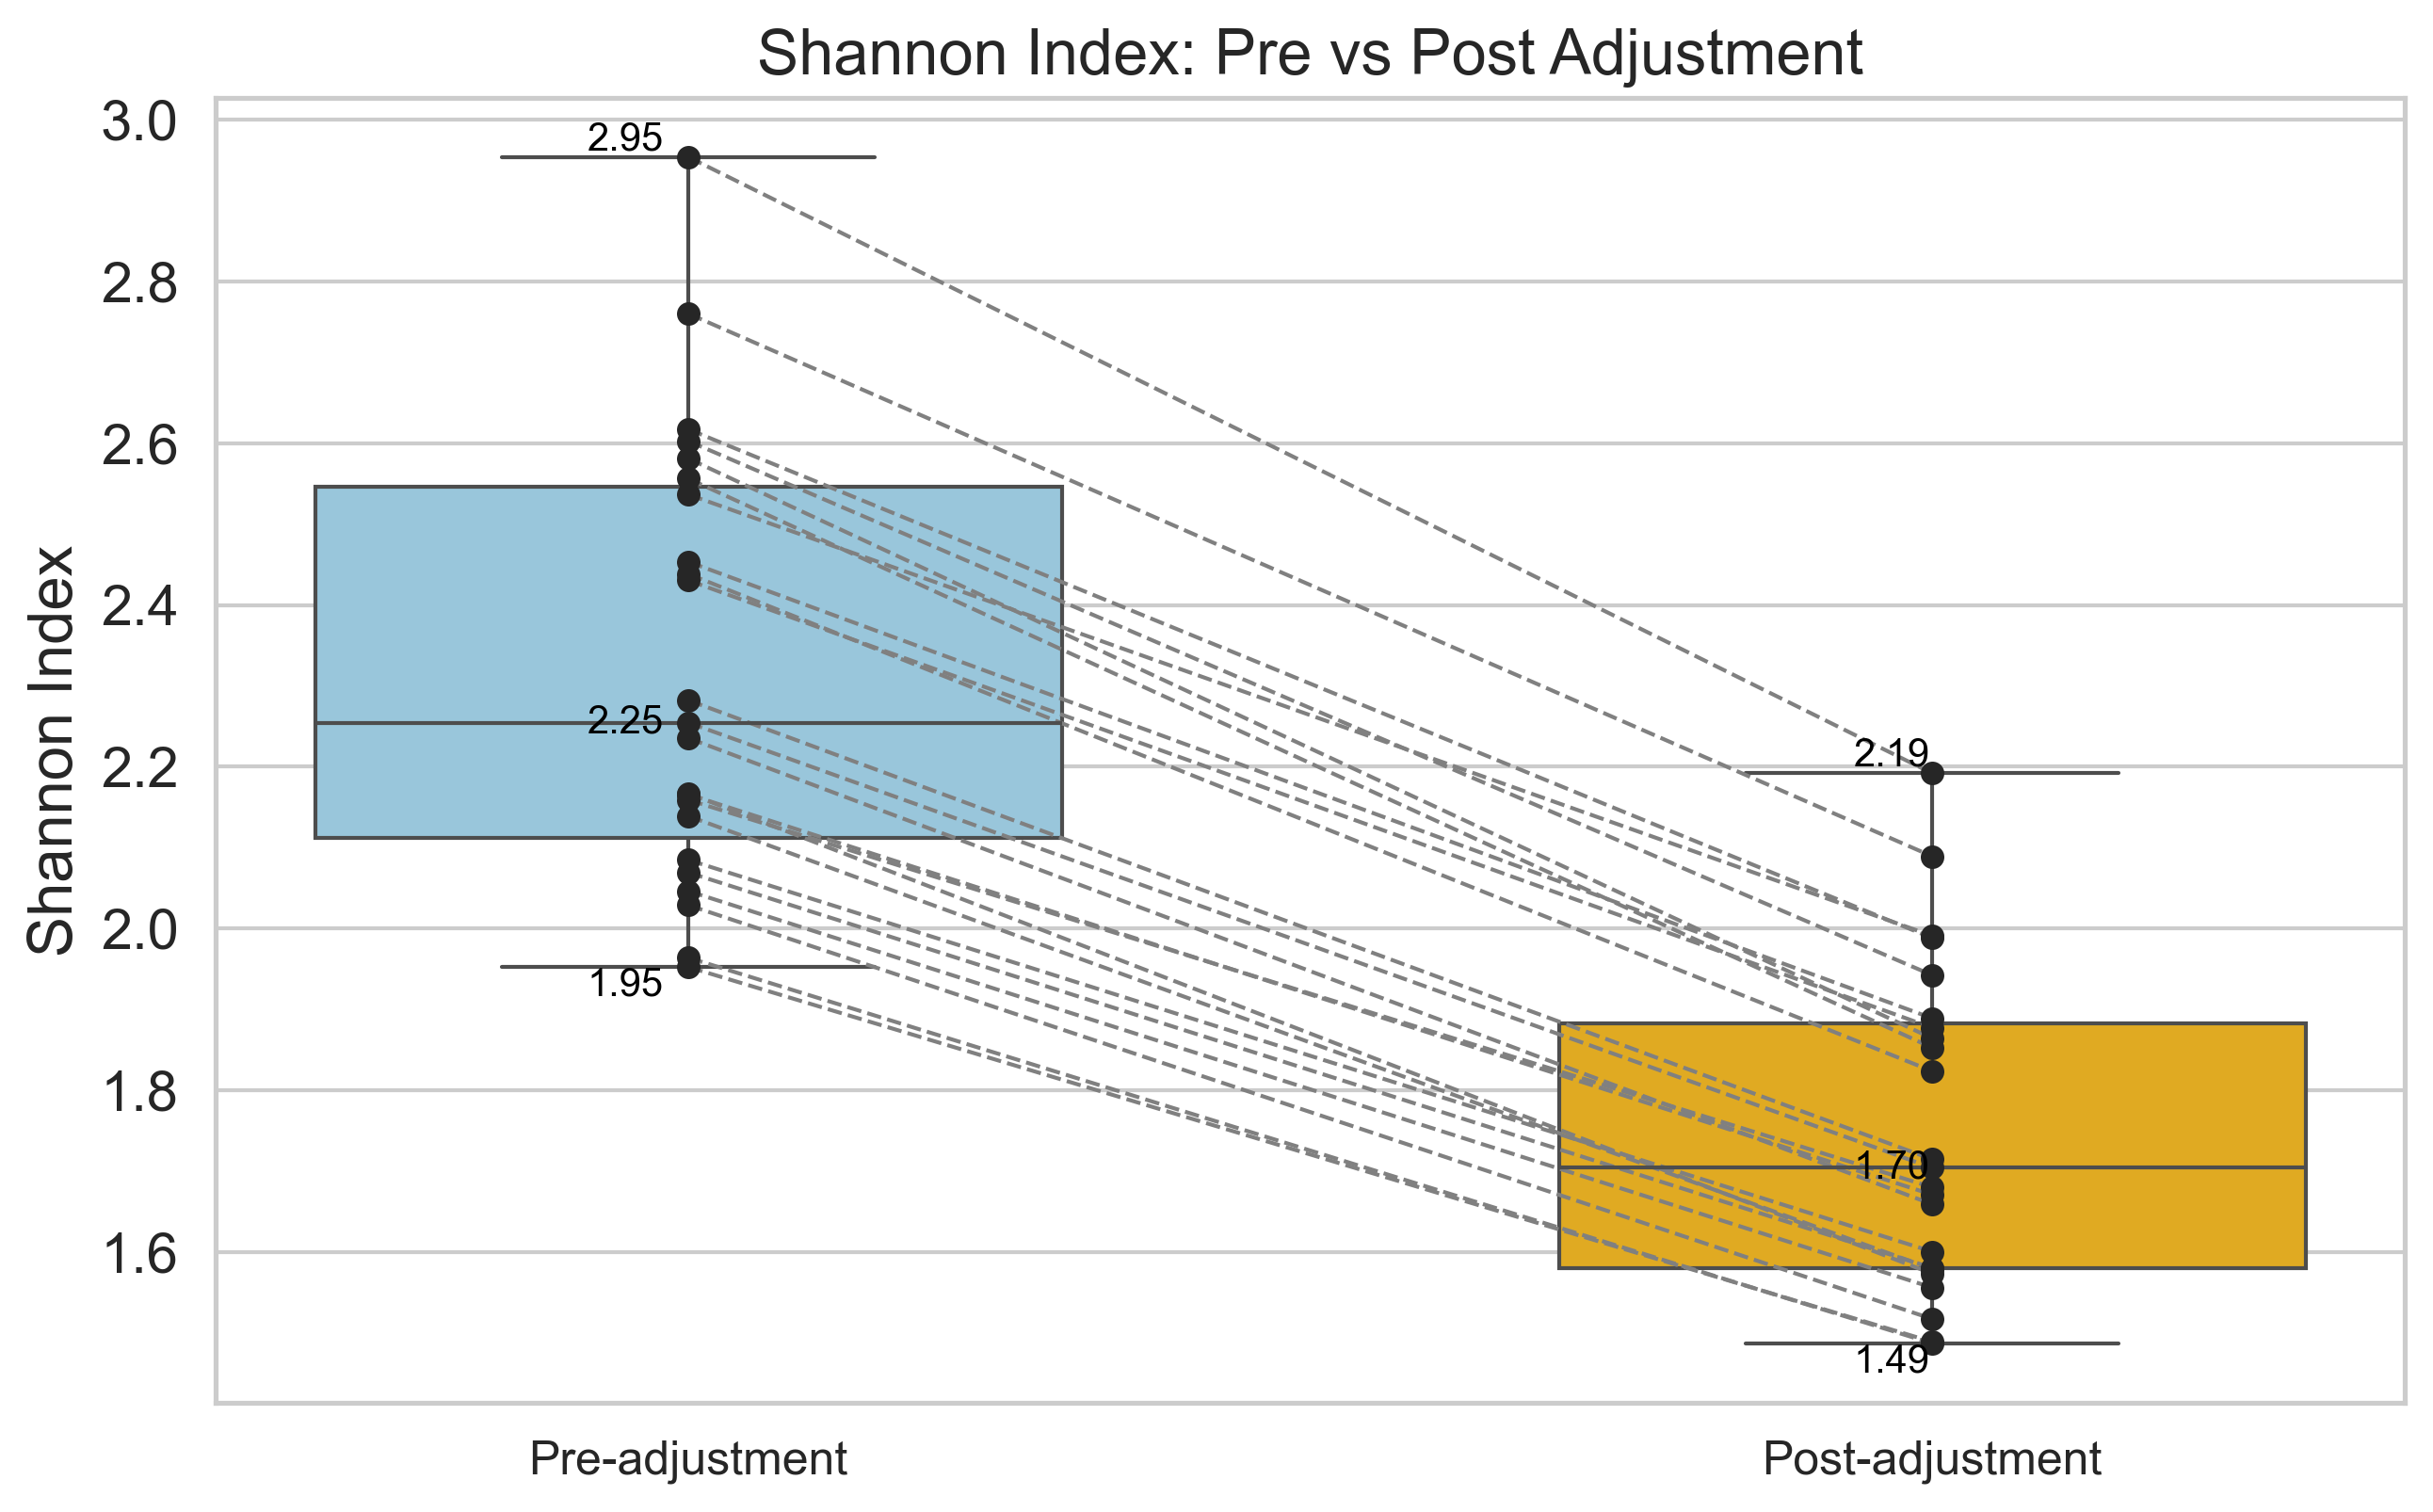
\includegraphics[width=0.8\textwidth]{Figures/shannon.png}
\caption{Shannon-Wiener Index: Pre vs Post Adjustment. The boxplots display the distribution of Shannon-Wiener index values across the complete dataset, before and after incorporating confidence levels. The dashed lines connect corresponding points between the two conditions, indicating the change in index values.}
\label{fig:shannon}
\end{figure}

As shown in Figure \ref{fig:shannon}, the median Shannon-Wiener index decreased from 2.25 to 1.70 after adjustment. This decrease suggests that the overall diversity within the studied communities is lower when accounting for the uncertainty in species identifications. The consistent downward shift in the index values highlights the impact of incorporating confidence levels, indicating that initial estimates of biodiversity may have been overestimated when assuming perfect species identification accuracy.


\subsubsection{Simpson Index}
The comparison of the Simpson index before and after adjustment is presented in Figure \ref{fig:simpson}. Contrary to the Shannon-Wiener index, the adjusted Simpson index values generally show a slight increase compared to the unadjusted values, which suggests a higher estimated diversity when the uncertainty in species identification is taken into account.

\begin{figure}[H]
\centering
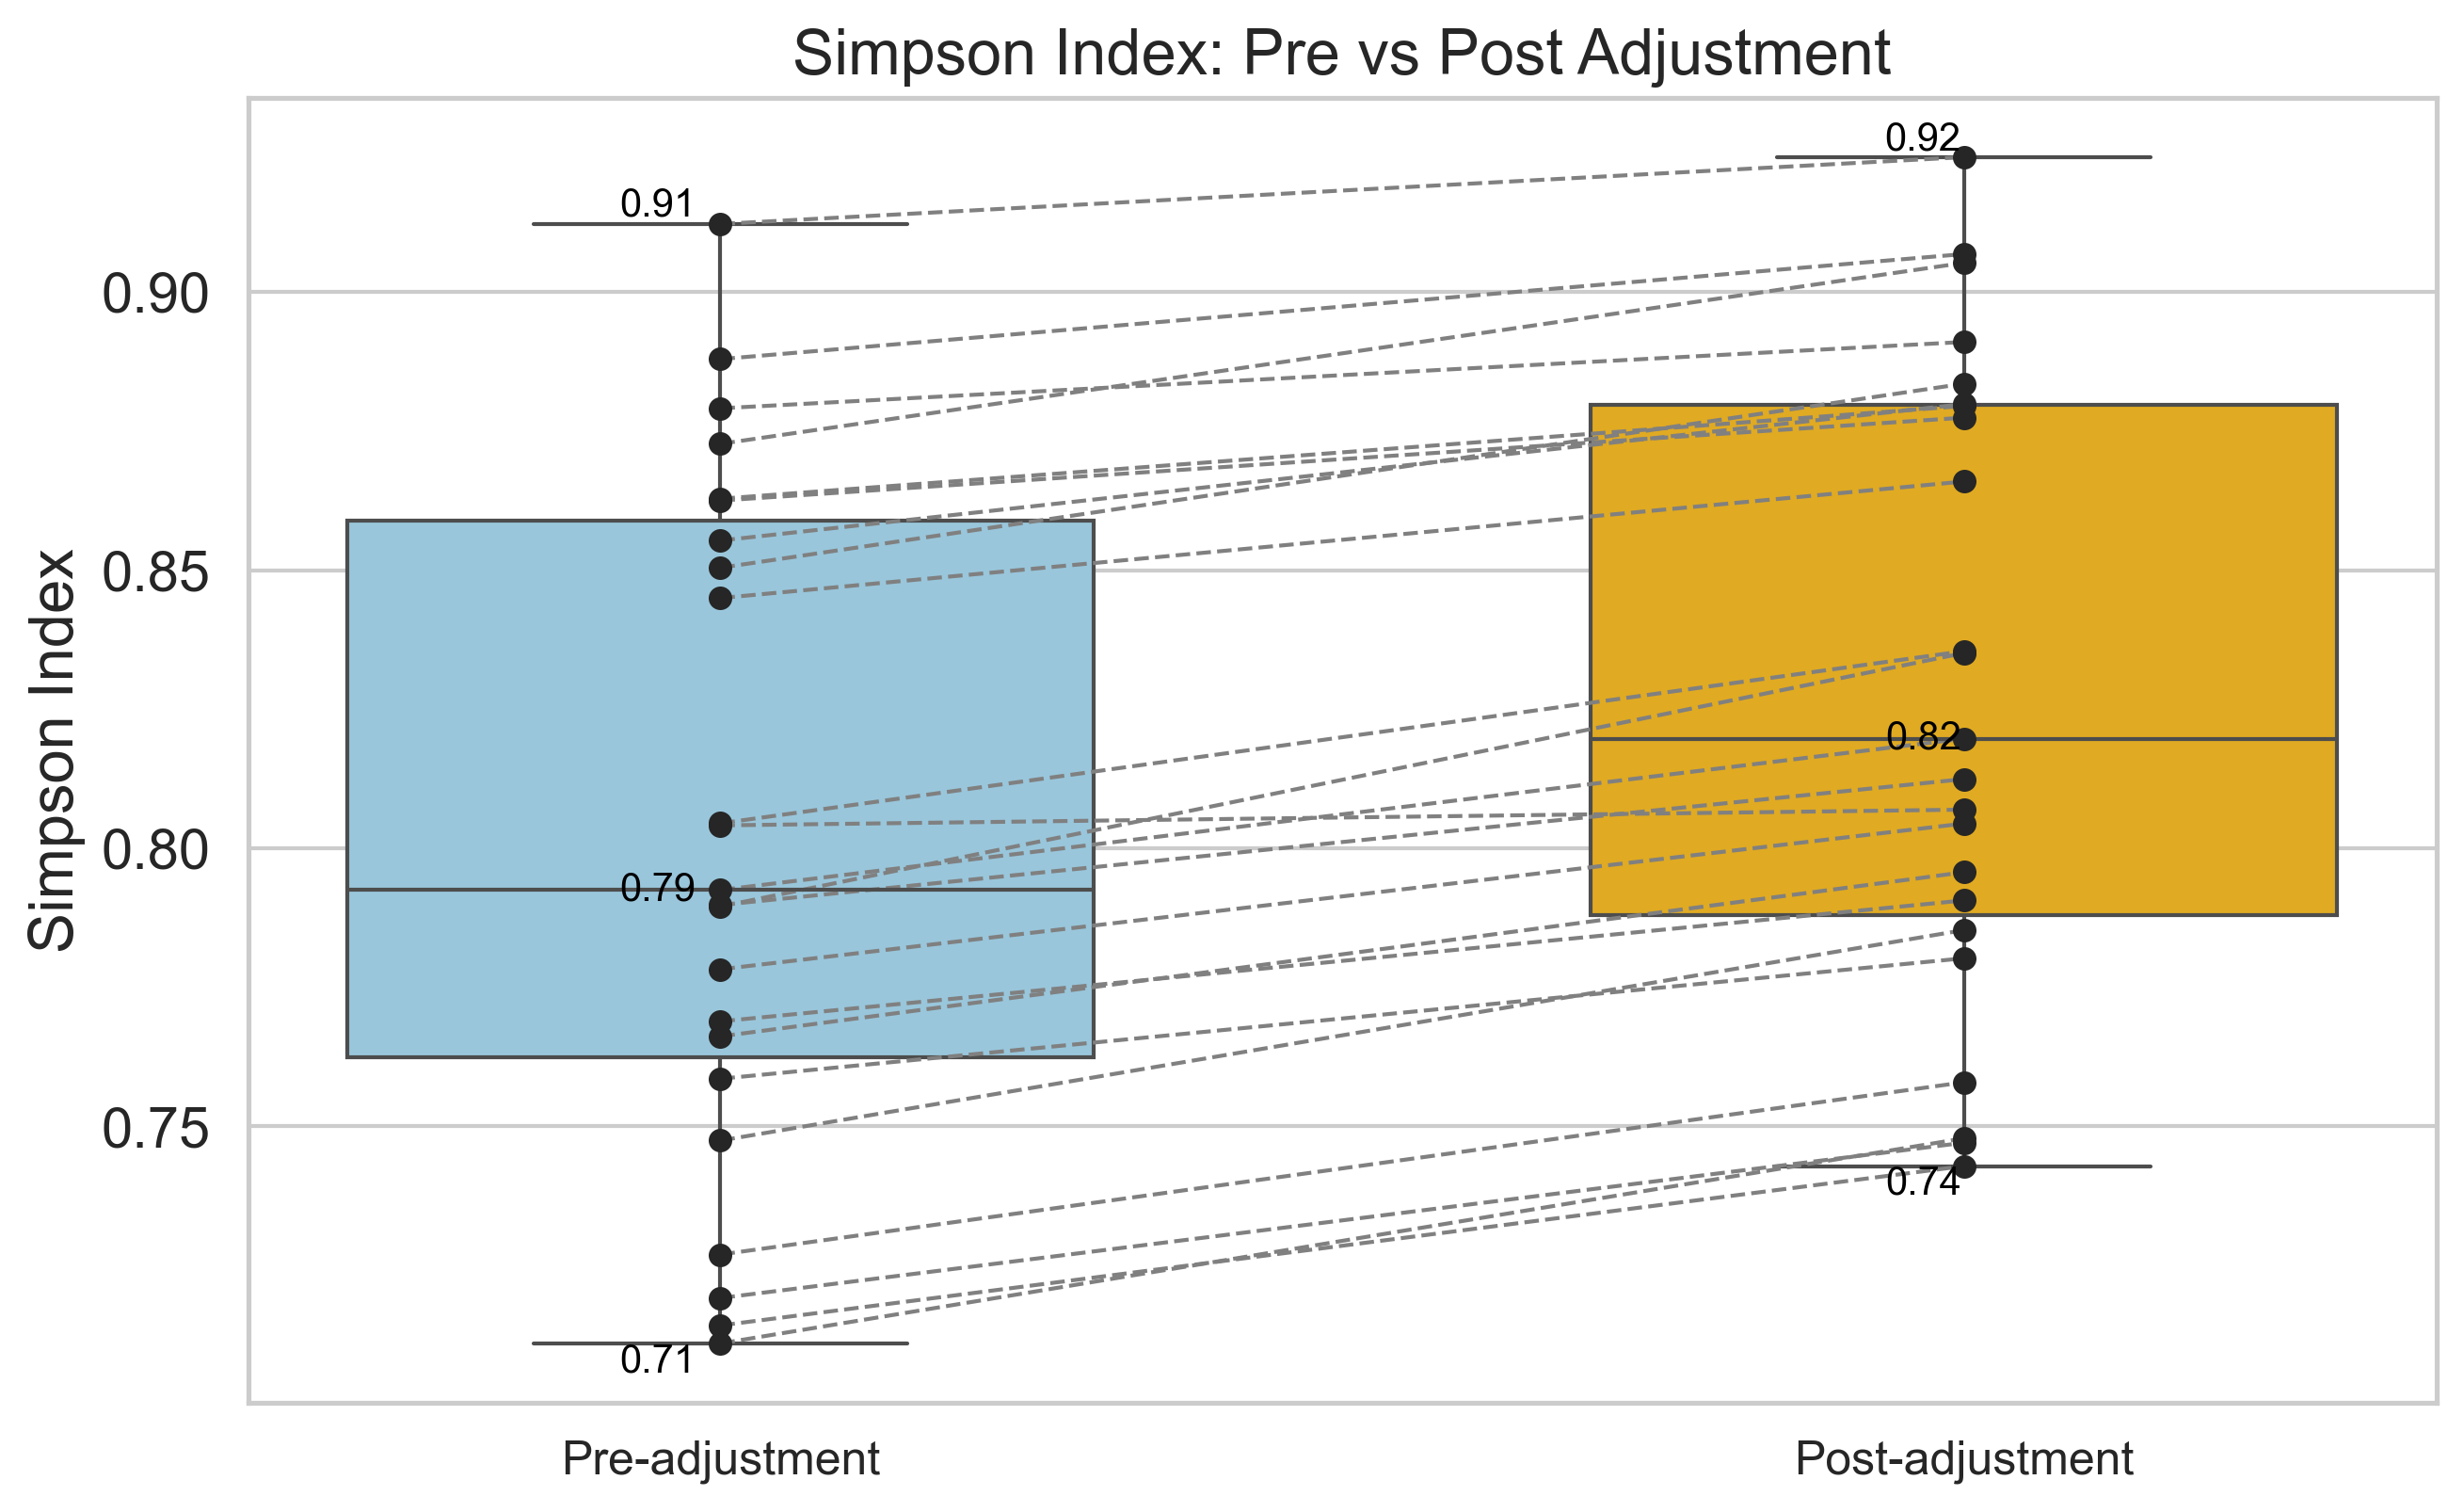
\includegraphics[width=0.8\textwidth]{Figures/simpson.png}
\caption{Simpson Index: Pre vs Post Adjustment. The boxplots display the distribution of Simpson index values across the complete dataset, before and after incorporating confidence levels. The dashed lines connect corresponding points between the two conditions, illustrating the changes in index values.}
\label{fig:simpson}
\end{figure}

As depicted in Figure \ref{fig:simpson}, the median Simpson index increased from 0.79 to 0.82 after adjustment. This increase indicates that when the confidence levels of species identifications are considered, the index reflects a slightly higher level of evenness within the community. This adjustment suggests that while some species might have been identified with lower confidence, their contribution to the overall diversity becomes more pronounced, leading to a more accurate representation of the community's evenness.

\subsubsection{Summary of Findings}
The results illustrate that adjusting for the confidence levels in species identification may affect the various diversity indices in different ways. In particular, the Shannon-Wiener index is estimated to decrease consistently after the adjustment. This result shows that this index reflects a more conservative estimation in the presence of uncertainty. The Simpson index slightly increases in value after the adjustment, indicating that it is much better to take into consideration the confidence levels for an improved estimation of evenness within the community. The contrasting results thus show that either underestimation or overestimation may occur with traditional diversity indices depending on the metric applied in the face of uncertainty in species identification. Therefore, these findings illustrate one critical reason to work confidence levels into diversity calculations, and thus enabling assessments of ecological communities that are more realistic and can be more reliable.





\subsection{Hill Numbers}

Hill numbers offer a unified framework for measuring species diversity that captures different aspects of diversity through varying the order $q$. The three Hill numbers considered here are:


\begin{itemize}
    \item Hill Number 0 (${}^0D$): Represents species richness, treating all species equally without considering their abundance.
    \item Hill Number 1 (${}^1D$): Equivalent to the exponential of the Shannon-Wiener index, accounting for both richness and evenness of species abundances.
    \item Hill Number 2 (${}^2D$): Equivalent to the inverse of the Simpson index, giving more weight to the most abundant species.
\end{itemize}

Figure \ref{fig:hill_numbers} presents a comparison of these Hill numbers before and after adjustments for confidence levels in species identification, using the entire dataset from December 2021 to April 2024.

\begin{figure}[H]
\centering
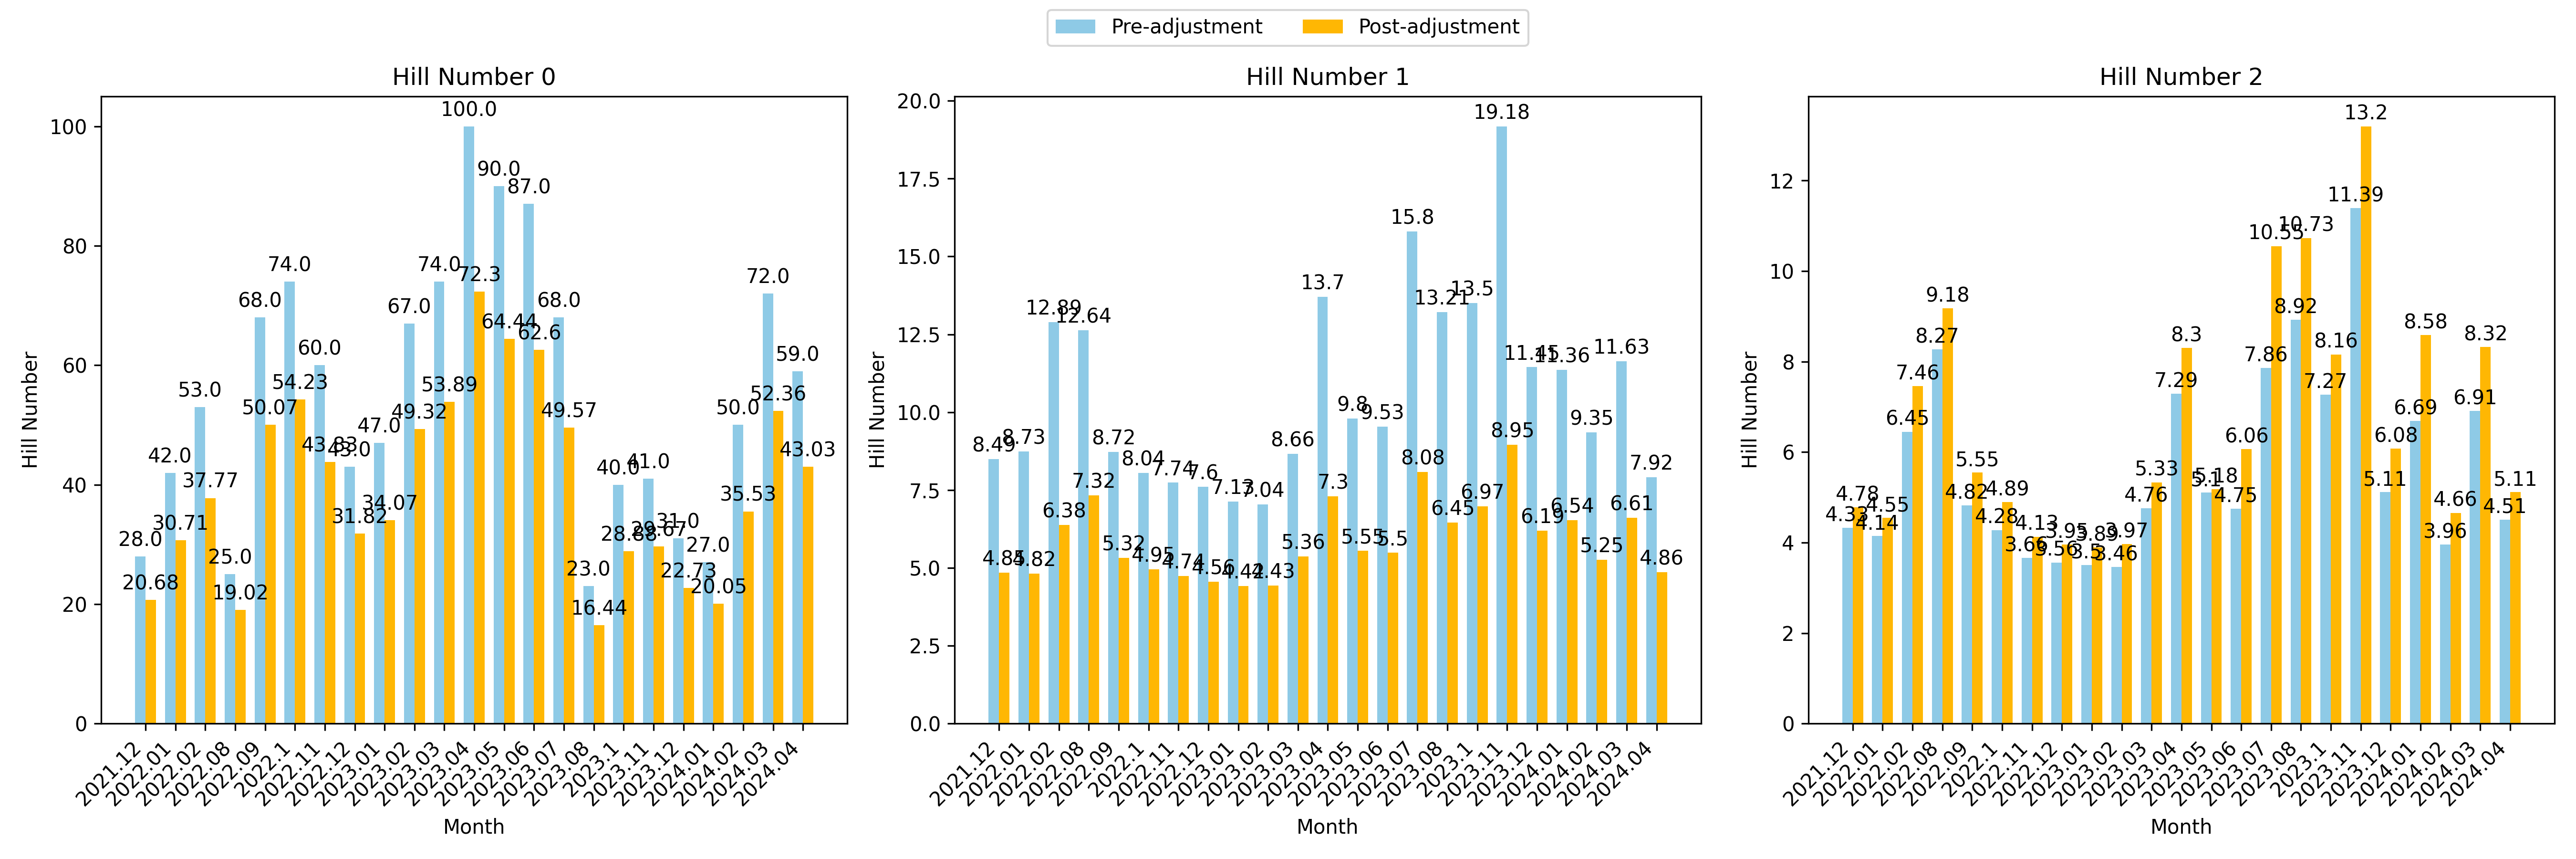
\includegraphics[width=1.0\textwidth]{Figures/Hill_Number.png}
\caption{Comparison of Hill Numbers (0, 1, 2 orders) before and after Adjustment. The bars represent Hill numbers across the entire dataset, with blue bars representing pre-adjustment values and red bars representing post-adjustment values.}
\label{fig:hill_numbers}
\end{figure}

The following observations are made from Figure \ref{fig:hill_numbers}:

\begin{itemize}
    \item \textbf{Hill Number 0 (Species Richness)}: Species richness showed a general decrease across most months, with the most significant reductions occurring during peak diversity periods. For instance, in April 2023, species richness dropped from 100.0 to 72.3, and in May 2023, it decreased from 90.0 to 64.44. This decrease suggests that incorporating confidence levels into species identification leads to a more conservative estimate of species richness.

    \item \textbf{Hill Number 1 (Shannon-Wiener Index)}: Similar trends were observed for Hill Number 1, where adjusted values were consistently lower than their pre-adjustment counterparts. For example, in August 2022, the index fell from 12.64 to 7.32, and in April 2023, it declined from 13.7 to 7.3. This indicates that when accounting for confidence levels, the perceived evenness of species abundances is reduced.

    \item \textbf{Hill Number 2 (Simpson Index)}: Interestingly, Hill Number 2 generally exhibited a decrease, though with some variability. For example, while most months showed a reduction, August 2022 recorded a slight increase from 8.27 to 9.18. This suggests that the dominance of the most abundant species may be less impacted or even slightly enhanced in certain months when adjustments are made for confidence levels.
\end{itemize}

Overall, the Hill numbers analysis suggests that incorporating confidence levels into diversity calculations tends to yield more conservative estimates of diversity, particularly for species richness and evenness. However, the impact on the dominance of abundant species (Hill Number 2) is more variable, reflecting the complex interaction between species abundance and identification confidence across different temporal scales.






\subsection{Analysis of $\gamma$ Diversity}

$\gamma$ diversity represents the overall diversity across all communities (or time periods) being studied. In this section, I compare the $\gamma$ diversity before and after adjustments, focusing on the Shannon-Wiener and Simpson indices, as well as species richness (Hill Number 0), all of which have been adjusted to account for species identification confidence.

\begin{figure}[H]
\centering
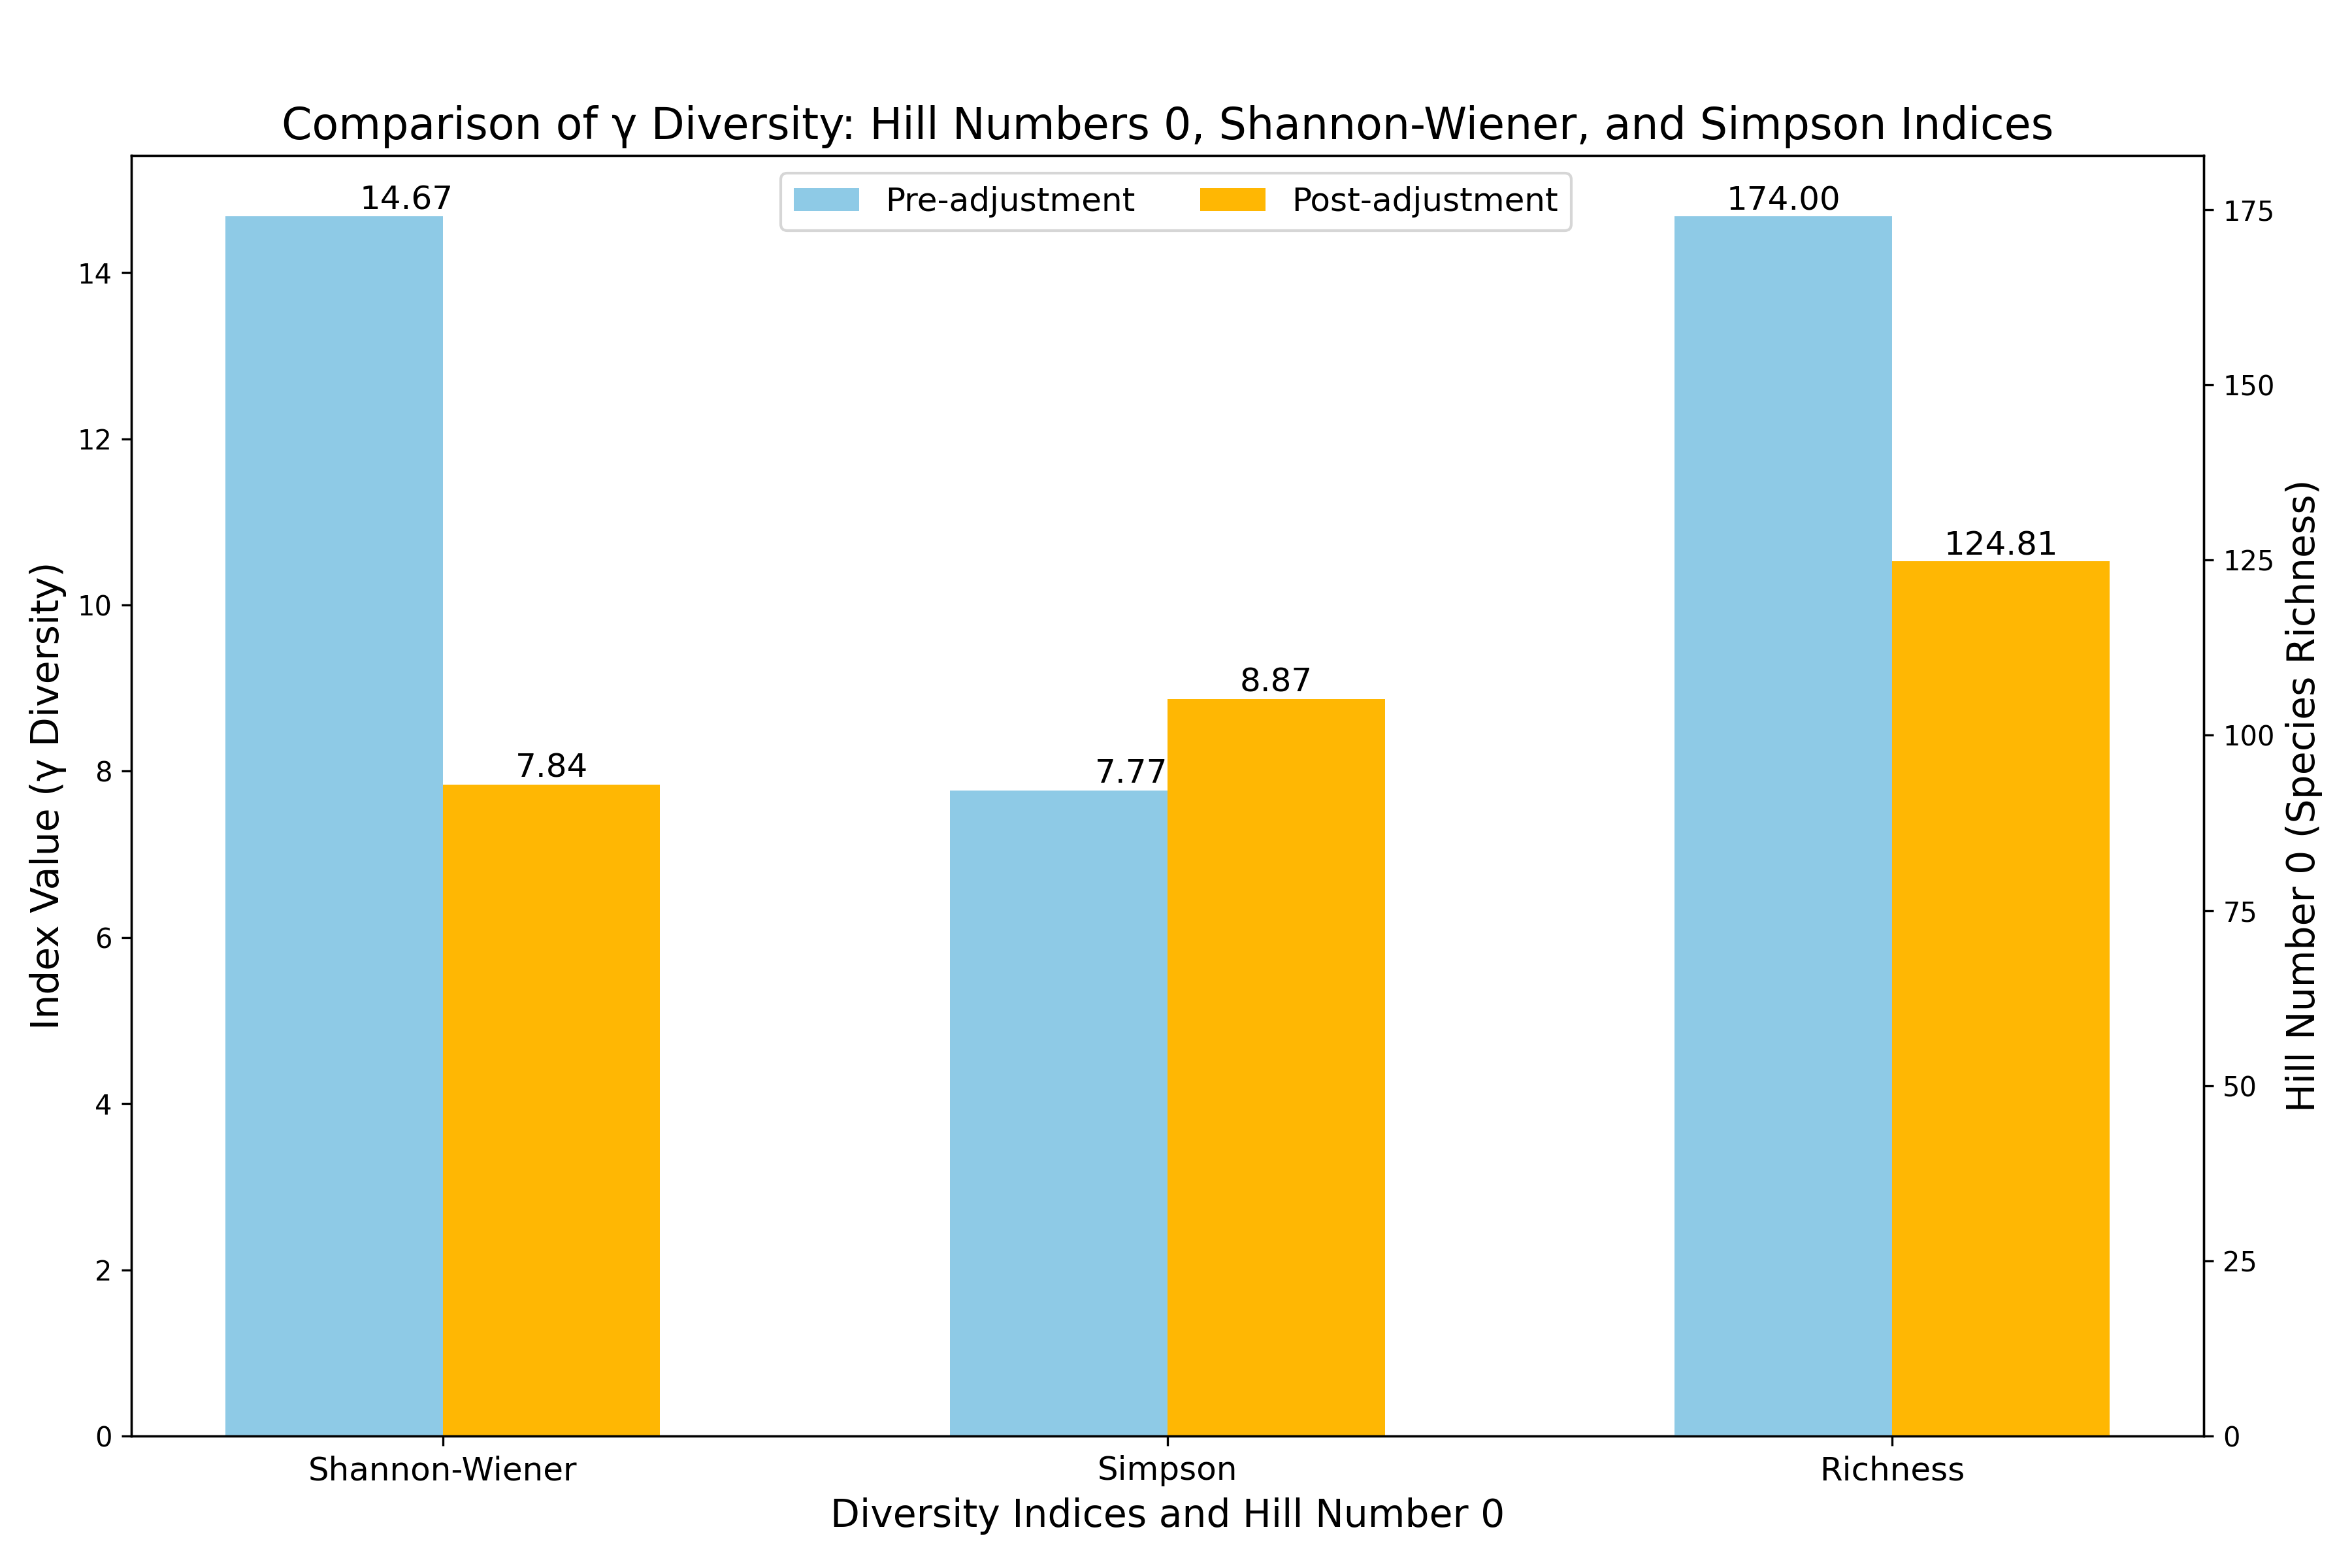
\includegraphics[width=0.8\textwidth]{Figures/gamma.png}
\caption{Comparison of $\gamma$ Diversity: Shannon-Wiener, Simpson Indices, and Species Richness (Hill Number 0) before and after Adjustment. The blue bars represent pre-adjustment values, and the red bars represent post-adjustment values.}
\label{fig:gamma_diversity}
\end{figure}

Figure \ref{fig:gamma_diversity} shows the comparison of the Shannon-Wiener, Simpson indices, and species richness, calculated for $\gamma$ diversity.

\begin{itemize}
    \item \textbf{Shannon-Wiener Index}: The Shannon-Wiener index decreased from 14.67 to 7.84 after adjustment. This significant reduction indicates that when confidence levels are taken into account, the overall diversity which combines all communities as a single community is substantially decreasing. It suggests that traditional calculations might overestimate diversity because it is not considering the uncertainty in species identification.
    
    \item \textbf{Simpson Index}: Conversely, the Simpson index increased from 7.77 to 8.87 after adjustment. This increase suggests that the evenness or dominance patterns within the community result in a higher overall diversity when accounting for confidence levels. The rise in the Simpson index can be resulting to a higher weighting of dominant species when confidence is taken into account.
    
    \item \textbf{Species Richness (Hill Number 0)}: The species richness also decreased from 174.00 to 124.81 after adjustment. This reduction reflects a more conservative estimate of the total number of species when considering the uncertainty in species identification.
\end{itemize}

Overall, these results suggest that accounting for uncertainty in species identification can lead to a more conservative estimate of species richness (as indicated by the Shannon-Wiener index and species richness). However, it may also highlight the dominance of certain species within the community (as indicated by the Simpson index). This analysis shows the importance of adjusting traditional diversity indices to consider the confidence into species identification. The result leads to a more robust understanding of biodiversity within the ecosystem being assessed.

\subsection{Analysis of $\beta$ Diversity}

$\beta$ diversity measures the variation in species composition between different communities or over different time periods, reflecting the degree of species turnover. In this study, I compared the $\beta$ diversity before and after adjustments for confidence levels, using the Shannon-Wiener and Simpson indices by using the formula introduced by \cite{jost2010independence}.

\begin{figure}[H]
\centering
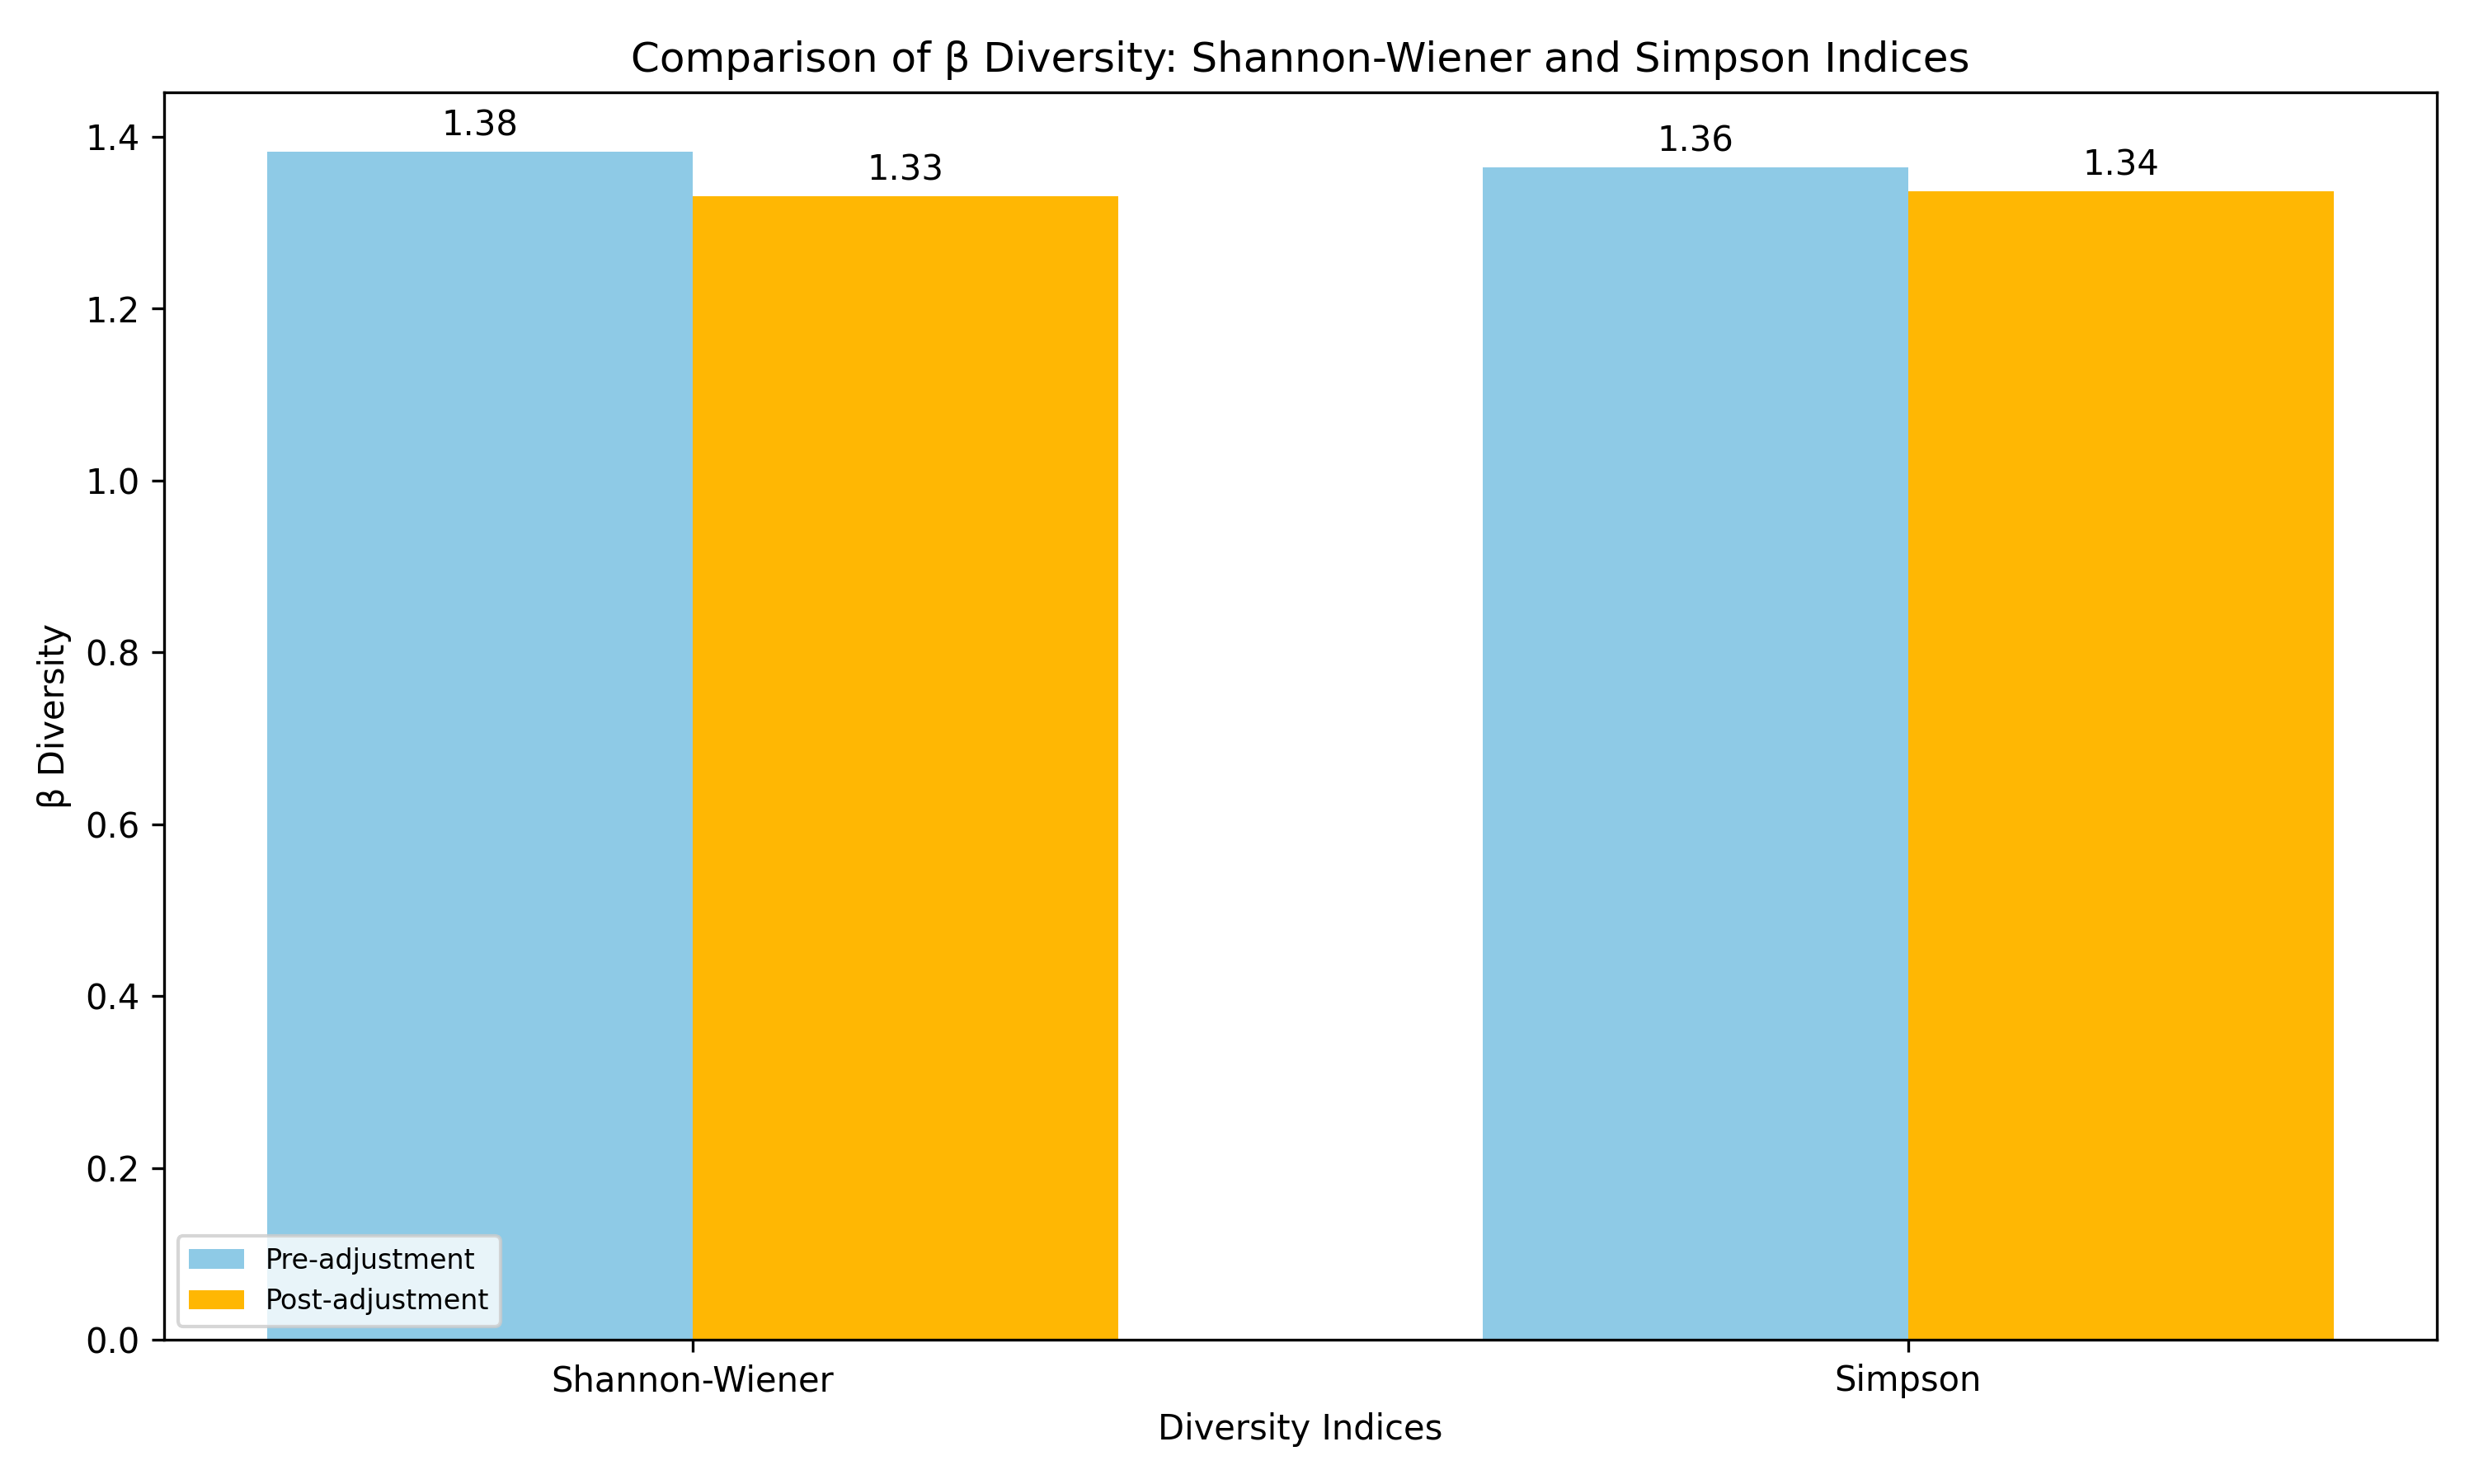
\includegraphics[width=0.8\textwidth]{Figures/beta_diversity.png}
\caption{Comparison of $\beta$ Diversity: Shannon-Wiener and Simpson Indices before and after Adjustment. The blue bars represent pre-adjustment values, and the red bars represent post-adjustment values.}
\label{fig:beta_diversity}
\end{figure}

Figure \ref{fig:beta_diversity} shows the $\beta$ diversity values calculated based on Shannon-Wiener and Simpson indices, before and after the correction.

\begin{itemize}
\item \textbf{Shannon-Wiener Index}: The $\beta$ diversity calculated from the Shannon-Wiener index shows a small decrease as a result of the adjustment, going from 1.38 to 1.33. The fact that this number diminishes indicates that with uncertainty in species identification, the turnover of species between the studied communities or time spans is just a bit less. This means that traditional calculations are inflated by the uncertainty about species, where it leads to just a bit overestimated variability in species composition.
\item \textbf{Simpson Index}: The $\beta$ diversity based on the Simpson index has dropped from 1.36 to 1.34 post-adjustment. This is an indication that the dominance patterns inside communities remain rather constant, because there is just a small drop in species turnover, even taking account of the confidence levels in identification. 
\end{itemize}

In general, these results suggest that accounting for confidence levels in species identification slightly reduces the estimated $\beta$ diversity. This implies that traditional indices tend to overestimate species turnover when they do not incorporate uncertainty in species identifications. As there is very little difference between the values before and after adjustment. This fact of robustness of the overall patterns of species turnover remains.






\subsection{Statistical Analysis Results}
To validate the effectiveness of the adjusted indices, several statistical tests were performed. The results, summarized in Table 1, indicate significant differences between the pre- and post-adjustment indices across all metrics.

\begin{table}[H]
\centering
\caption{Statistical Analysis of Pre- and Post-Adjustment Indices}
\begin{tabular}{lrrrrr}
\hline
\textbf{Metric} & \textbf{T-statistic} & \textbf{P-value} & \textbf{Cohen's d} & \textbf{Spearman's $\rho$} & \textbf{Kendall's $\tau$} \\
\hline
Shannon-Wiener & 32.21 & 5.25e-20 & -2.39 & 0.9506 & 0.8419 \\
Simpson        & -12.43 & 2.01e-11 & 0.43  & 0.9763 & 0.8814 \\
Hill Number 0  & 11.65 & 7.05e-11 & -0.78 & 0.9995 & 0.9960 \\
Hill Number 1  & 11.89 & 4.71e-11 & -2.00 & 0.9506 & 0.8419 \\
Hill Number 2  & -7.20 & 3.26e-07 & 0.40  & 0.9763 & 0.8814 \\
\hline
\end{tabular}
\end{table}

The T-statistic and P-value indicate statistically significant differences between the pre- and post-adjustment indices for all diversity metrics. The Cohen's d values suggest that the Shannon-Wiener index and Hill Number 1 have large negative effect sizes. This indicates a substantial decrease in diversity post-adjustment. In contrast, both the Simpson index and Hill Number 2 have a moderate positive effect size. This shows that evenness increases and dominance decreases after adjustment. The values of Spearman's $\rho$ and Kendall's $\tau$ are high between pre- and post-adjustment regarding order consistency and highlight a good robustness of these indices after adjustment. This shows that the order of the index adjustment remains basically the same.



\section{Discussion}

\subsection{Interpretation of Results}
Several key findings have arisen from adjusting diversity indices for uncertainty in species identification. The Shannon-Wiener index, which considers both richness and evenness, dropped drastically after introducing the confidence. This suggest that assuming the confidence of the species identification, the perceived diversity within the studied communities is less than estimated. This result supports the hypothesis that traditional diversity indices overestimate biodiversity due to the lack of consideration for uncertainty in automated identification tools. However, the Simpson index increased with this change. This indicates that although species richness might be lower, the patterns of evenness or dominance are much clearer when accounting for confidence levels. Indeed, the rise in the Simpson index could indicate that dominant species are more heavily weighted in the overall diversity estimate.

The Hill number approach is different from those of above; the Hill Number 0, i.e., the count of species richness, declined across all months surveyed, which validates the premise that a confidence-based estimate produces a conservative estimate of species diversity. Indeed, also even Hill Number 1, which is the exponential of Shannon-Wiener index, decreased when accounting for uncertainty. This result implies that evenness decreases. However, the Hill Number 2 gave more varied results with some months showing even higher values than in the other cases, suggesting that the dominance of the abundant species can become even clearer in certain case \citep{magurran2004measuring}.


\subsection{Implications for Ecological Studies}
These findings have important implications for ecological studies that rely on automated species identification systems. The overestimation or underestimation of biodiversity due to unaccounted uncertainty can lead to incorrect conclusions about the health and stability of ecosystems. By incorporating confidence levels into the calculation of diversity indices, researchers can obtain a more accurate and robust understanding of species diversity, which is crucial for effective conservation and management strategies \citep{arponen2012prioritizing}.

Furthermore, the variation observed in Hill Number 2 across different months highlights the dynamic nature of species dominance within ecosystems. This variability suggests that the impact of adjusting diversity indices for confidence levels may depend on temporal factors, such as seasonal changes or fluctuations in species populations. Understanding these temporal dynamics is essential for accurately monitoring biodiversity over time and for identifying periods of significant ecological change.

The observed changes in $\gamma$ and $\beta$ diversity also underscore the importance of adjusting traditional indices. The decrease in $\gamma$ diversity after adjustment suggests that the overall species diversity across the study site is lower when confidence is factored in. This has implications for regional biodiversity assessments, where overestimation of diversity could lead to the misallocation of conservation resources. Similarly, the slight decrease in $\beta$ diversity indicates that species turnover between communities or time periods might be less pronounced than previously thought, affecting how we understand species distribution patterns.


\subsection{Limitations and Future Work}
While my study contributes some value to the insight about introducing confidence levels in the diversity indices, there are still some areas that could be studied further. One critical area is in the fine-tuning of the confidence scores generated by algorithms such as BirdNET. Currently, these are relative measures and do not directly translate into actual probabilities. This work shall focus on the calibration of such confidence scores, so that make the measures reflect the true likelihood in species identification. This may include the development of machine learning models in which confidence scoring is conditioned on some different factors, such as acoustic signal quality, environmental conditions, the existence of same species individuals within a geographic area, quality of detecting equipment.

Another interesting development would be to use these modified indices in other ecological contexts for the monitoring of biodiversity in different habitats or under different environmental pressures. By comparing such data across a wide range of different ecological conditions, it is possible to measure the performance of adjusted indices and get a better understanding of generalizability and limitations. It might be useful also for the more accurate tracking over time of changes in species diversity under long-term biodiversity monitoring programs as input necessary for any species conservation planning. Relative abundances calculated in my dataset show that some birds have very small abundances and it is close to zero. The heterogeneity of the sample might explain this reason of some change of the indices. In my analysis, I focused on detected time as a significant factor. I divided different communities by month and conducted corresponding studies. From another perspective, communities could also be divided based on geographical information. This is another method to check whether the modified index can still measure and explain changes in species diversity accurately.

Lastly, additional statistical methods could include other Bayesian approaches for further analyses on how uncertainty affects assessments of biodiversity. In this regard, Bayesian methods is also a feasible way to analysis the change of indices. Starting with the most basic Bayesian formula, it seems to get a suitable result while considering the uncertainty of species identification.


\section{Conclusion}
My work has proved how important it is to include some level of uncertainty associated with the identity of species when calculating biodiversity indices. The modifications applied to the Shannon-Wiener and Simpson indices, along with modifications to the Hill numbers, have led to a better representation of the actual species diversity occurring in the analyzed communities. These findings obviously reveal potential biases of traditional indices and may call for more sophisticated approaches that could eventually include confidence levels into the assessment of biodiversity. Looking back at the previous hypothesis in the introduction, my research shows that traditional diversity indices like the Shannon and Simpson indices often overestimate species diversity. By analyzing the Hill Number of effective species and examining $\gamma$ and $\beta$ diversity, I found that introducing confidence into the index can better reflect the true species diversity. This approach also allows the diversity index to be more closely linked with ecosystem diversity.


In general, with automatic species identification tools are more widely used in ecological research, approaches developed in my study will be useful for ensuring accuracy and trustworthiness of biodiversity data towards more informed conservation and management decisions.


\section*{Data and Code Availability}
The data and codes that support the findings of my report are available from the repositories: \href{https://github.com/Bowen12580/CMEEMaster}{https://github.com/Bowen12580/CMEEMaster}



\newpage





\bibliographystyle{agsm}
\bibliography{ref}


\end{document}